\documentclass{book}
\usepackage{physics}
\usepackage{graphicx}
\usepackage{caption}
\usepackage{amsmath}
\usepackage{bm}
\usepackage{framed}
\usepackage{authblk}
\usepackage{empheq}
\usepackage{amsfonts}
\usepackage{esint}
\usepackage[makeroom]{cancel}
\usepackage{dsfont}
\usepackage{centernot}
\usepackage{mathtools}
\usepackage{bigints}
\usepackage{amsthm}
\theoremstyle{definition}
\newtheorem{defn}{Definition}[section]
\newtheorem{prop}{Proposition}[section]
\newtheorem{rmk}{Remark}[section]
\newtheorem{thm}{Theorem}[section]
\newtheorem{exmp}{Example}[section]
\newtheorem{prob}{Problem}[section]
\newtheorem{sln}{Solution}[section]
\newtheorem*{prob*}{Problem}
\newtheorem{exer}{Exercise}[section]
\newtheorem*{exer*}{Exercise}
\newtheorem*{sln*}{Solution}
\usepackage{empheq}
\usepackage{tensor}
\usepackage{xcolor}
%\definecolor{colby}{rgb}{0.0, 0.0, 0.5}
\definecolor{MIT}{RGB}{163, 31, 52}
\usepackage[pdftex]{hyperref}
%\hypersetup{colorlinks,urlcolor=colby}
\hypersetup{colorlinks,linkcolor={MIT},citecolor={MIT},urlcolor={MIT}}  



\newcommand*\widefbox[1]{\fbox{\hspace{2em}#1\hspace{2em}}}

\newcommand{\p}{\partial}
\newcommand{\R}{\mathbb{R}}
\newcommand{\C}{\mathbb{C}}
\newcommand{\lag}{\mathcal{L}}
\newcommand{\nn}{\nonumber}
\newcommand{\ham}{\mathcal{H}}
\newcommand{\M}{\mathcal{M}}
\newcommand{\I}{\mathcal{I}}
\newcommand{\K}{\mathcal{K}}
\newcommand{\F}{\mathcal{F}}
\newcommand{\w}{\omega}
\newcommand{\lam}{\lambda}
\newcommand{\al}{\alpha}
\newcommand{\be}{\beta}
\newcommand{\x}{\xi}

\newcommand{\G}{\mathcal{G}}

\newcommand{\f}[2]{\frac{#1}{#2}}

\newcommand{\ift}{\infty}

\newcommand{\lp}{\left(}
\newcommand{\rp}{\right)}

\newcommand{\lb}{\left[}
\newcommand{\rb}{\right]}

\newcommand{\lc}{\left\{}
\newcommand{\rc}{\right\}}


\newcommand{\V}{\mathbf{V}}
\newcommand{\U}{\mathcal{U}}
\newcommand{\Id}{\mathcal{I}}
\newcommand{\D}{\mathcal{D}}
\newcommand{\Z}{\mathcal{Z}}

%\setcounter{chapter}{-1}






\usepackage{subfig}
\usepackage{listings}
\captionsetup[lstlisting]{margin=0cm,format=hang,font=small,format=plain,labelfont={bf,up},textfont={it}}
\renewcommand*{\lstlistingname}{Code \textcolor{violet}{\textsl{Mathematica}}}
\definecolor{gris245}{RGB}{245,245,245}
\definecolor{olive}{RGB}{50,140,50}
\definecolor{brun}{RGB}{175,100,80}

%\hypersetup{colorlinks,urlcolor=colby}
\lstset{
	tabsize=4,
	frame=single,
	language=mathematica,
	basicstyle=\scriptsize\ttfamily,
	keywordstyle=\color{black},
	backgroundcolor=\color{gris245},
	commentstyle=\color{gray},
	showstringspaces=false,
	emph={
		r1,
		r2,
		epsilon,epsilon_,
		Newton,Newton_
	},emphstyle={\color{olive}},
	emph={[2]
		L,
		CouleurCourbe,
		PotentielEffectif,
		IdCourbe,
		Courbe
	},emphstyle={[2]\color{blue}},
	emph={[3]r,r_,n,n_},emphstyle={[3]\color{magenta}}
}


\begin{document}
\begin{titlepage}\centering
 \clearpage
 \title{{\textsc{\textbf{CLASSICAL MECHANICS}}}\\ \smallskip - A Quick Review - \\}
 \author{\bigskip Huan Q. Bui}
  \affil{B.A., COLBY COLLEGE (2021) $\,$\\  
  	MASSACHUSETTS INSTITUTE OF TECHNOLOGY}
 \date{June 15, 2021 -   \today}
 \maketitle
 \thispagestyle{empty}
\end{titlepage}




\noindent \textbf{Preface}


$\,$\\


\noindent Greetings, \\

This article contains some of my preparation for the upcoming Ph.D. qualifying exam in classical mechanics. There will be some theory as well as examples and problems. I'm only covering the more ``advanced'' content from undergraduate courses such as Lagrangian and Hamiltonian mechanics and so on. Familiarity with intermediate classical mechanics is assumed. \\

\noindent Enjoy! (I guess)



\newpage







\chapter{Theory}






\section{Lagrangian Mechanics}

The \textbf{Lagrangian} for a conservative system is given by 
\begin{equation*}
\lag = T - U
\end{equation*}
where $T$ is the kinetic energy and $U$ is the potential energy. \\

The $n$ parameters $q_1,\dots,q_n$ are said to be \textbf{generalized coordinates} for an $N$-particle system if every particle's position $\mathbf{r}_i$ can be expressed as a function of $q_1,\dots,q_n$ (and time $t$) and if $n$  is the smallest number that allows the system to be described this way ($n$ must be minimal). \\

In 3D, if $n< 3N$, then the system is said to be \textbf{constrained}. $q_1,\dots,q_n$ are said to be \textbf{natural} if the functional relationships between the $q_i$'s and $\mathbf{r}_i$ are time-independent. \\


The number of \textbf{degrees of freedom} of a system is the number of coordinates that can be independently varied. If the degrees of freedom is equal to the the number of generalized coordinates (which is ``normal'') then the system is said to be \textbf{holonomic}. An example of a nonholonomic system is a ball rolling on a flat table without slipping (see Taylor's \textit{Classical Mechanics}, Chapter 7 for more details) or a mass on the surface of a sphere in a gravitational field. \\


Holonomic (i.e. ``normal'') systems satisfy the \textbf{Euler-Lagrange equations}:
\begin{equation*}
\f{d}{dt}\f{\p \lag}{\p \dot{q}_i} = \f{\p \lag}{\p {q}_i}.
\end{equation*} 
The Euler-Lagrange equations are equivalent to \textbf{Hamilton's principle}, which states that the actual path which a particle follows between two points $1$ and $2$ in a given time interval $[t_1,t_2]$ is such that the action 
\begin{equation*}
S = \int^{t_2}_{t_1} \lag\,dt
\end{equation*}
is stationary. \\


For each generalized coordinate $q_i$, we have a \textbf{generalized momentum} $p_i$, given by
\begin{equation*}
p_i = \f{\p \lag}{\p \dot{q}_i}.
\end{equation*}
It easy to see that, from the Euler-Lagrange equations, $p_i$ is constant, or \textbf{conserved}, whenever $\p\lag / \p q_i = 0$. In this case, we say that the generalized coordinate $q_i$ is \textbf{ignorable} or \textbf{cyclic}.  \\

This can be stated the following way: $p_i$ is a constant of motion if the conjugate coordinate $q_i$ is cyclic. This is basically \textbf{Noether's Theorem}. 






\section{Hamiltonian Mechanics}



The \textbf{Hamiltonian} can be obtained from the Lagrangian via the Legendre transformation. The Hamiltonian is defined as
\begin{equation*}
\mathcal{H} = \sum_{i=1}^n p_i  \dot{q}_i - \lag.
\end{equation*}


The Hamiltonian is said to be \textbf{conserved} if $\p \lag/\p t = -\p \ham/\p t = 0$. If the coordinates $q_1,\dots,q_n$ are natural (recall: ``natural'' = time-independent with respect to positions) then the Hamiltonian is equal to the \textbf{total energy} of the system. \\




For each $i = 1,2,\dots, n$, the time evolution of the system is given by the \textbf{Hamilton's equations}:
\begin{equation*}
\dot{q}_i = \f{\p \mathcal{H}}{ \p p_i} \quad \text{and} \quad \dot{p}_i = -\f{\p \ham}{\p q_i}.
\end{equation*}
An important identity:
\begin{equation*}
\f{\p \lag}{\p t} = - \f{\p \ham}{\p t}.
\end{equation*}



A somewhat more advanced but related topic is \textbf{Poisson brackets}. Given the canonical coordinates $p_i,q_i$ and two functions $f(q_i,p_i,t),g(q_i, p_i,t)$, the Poisson bracket of $f,g$ is defined by 
\begin{equation*}
\{ f,g \} = \sum_i \lp \f{\p f}{\p q_i} \f{\p g}{\p p_i} - \f{\p f}{\p p_i} \f{\p g}{\p q_i} \rp.
\end{equation*} 



Poisson brackets for the canonical coordinates are
\begin{equation*}
\{q_i, q_j \} = 0, \quad \{ p_i ,p_j \} = 0, \quad \{ q_i , p_i \} = \delta_{ij}
\end{equation*}



Hamilton's equations of motion can be formulated in terms of Poisson brackets. Let $\phi = \phi(p,q,t)$ be some function on the solution's trajectory-manifold. Then we have
\begin{equation*}
\f{d}{dt}\phi(p,q,t) = \f{\p \phi}{\p q} \f{d q}{dt} + \f{\p \phi }{\p p} \f{d p}{dt} + \f{\p \phi}{\p t}.
\end{equation*}
Let $p = p(t)$ and $q = q(t)$ be solutions to the Hamilton's equations, i.e., $\dot{p} = -\p \ham / \p q$ and $\dot{q} = \p \ham  / \p p$. From the definition of Poisson brackets we can identify:
\begin{equation*}
\dot{p} = -\f{\p \ham}{\p q} = \{ p,\ham \} \quad \text{and} \quad \dot{q} = \f{\p \ham}{\p p} = \{ q,\ham \}.
\end{equation*}
Thus, from the chain rule above we find that, for any function $\phi = \phi(p,q,t)$,
\begin{equation*}
\f{d}{dt}\phi(p,q,t) = \f{\p \phi}{\p q} \f{\p \ham}{\p p} - \f{\p \phi}{\p p}\f{\p \ham}{\p q} + \f{\p \phi}{\p t} = \{ \phi,\ham \} + \f{\p \phi}{\p t}.
\end{equation*}


\section{Two-Body Central-Force Problems}

Given a two-body problem, we can re-write it in terms of the \textbf{relative coordinate} $\textbf{r}$ and \textbf{CM coordinate} $\textbf{R}$:
\begin{equation*}
\textbf{r} = \textbf{r}_1 - \textbf{r}_2 \quad \text{and} \quad \textbf{R}  = \f{m_1 \textbf{r}_1 + m_2 \textbf{r}_2}{m_1+m_2}.
\end{equation*}
We also introduce the \textbf{reduced mass} $mu$:
\begin{equation*}
\mu = \f{m_1 m_2}{m_1 + m_2}.
\end{equation*}
The {kinetic energy} is then given by 
\begin{equation*}
T = \f{1}{2}m_1 \dot{\textbf{r}}_1^2 + \f{1}{2}m_2 \dot{\textbf{r}}_2^2 = \f{1}{2}M\dot{\textbf{R}}^2 + \f{1}{2}\mu \dot{\textbf{r}}^2
\end{equation*}
where $M$ is the total mass. The \textbf{Lagrangian} can then be decomposed into the CM Lagrangian plus the relative Lagrangian:
\begin{equation*}
\lag = T - U(r) = \f{1}{2}M\dot{\textbf{R}}^2 + \lp \f{1}{2}\mu \dot{\textbf{r}}^2 - U(r) \rp =  \lag_\text{CM} + \lag_{\text{rel}}
\end{equation*}

By going into the CM frame, $\lag_\text{CM} = 0$, and we basically have a 1-body problem because $\dot{\textbf{R}} = 0$. In this frame, the angular momentum (which is conserved) can be easily calculated:
\begin{equation*}
L = \textbf{r}_1 \times \textbf{p}_1 + \textbf{r}_2 \times \textbf{p}_2 = m_1 \textbf{r}_1 \times \dot{\textbf{r}}_1 +  m_2 \textbf{r}_2 \times \dot{\textbf{r}}_2  = \dots = \textbf{r} \times \mu \dot{\textbf{r}}. 
\end{equation*}
By going into polar coordinates, we can write $\dot{\textbf{r}}$ in terms of $r$ and the polar angle $\phi$. The CM Lagrangian becomes
\begin{equation*}
\lag_\text{CM} = \f{1}{2}\mu \lp \dot{r}^2 + r^2 \dot{\phi}^2 \rp - U(r).
\end{equation*}
This Lagrangian does not depend on $\phi$, so $\phi$ is ignorable, and so $\p \lag / \p \dot{\phi}$, which is the \textbf{angular momentum}, is conserved. This quantity is 
\begin{equation*}
\boxed{\f{\p \lag}{\p \dot{\phi}} = \mu r^2 \dot{\phi} = l = \text{constant}}
\end{equation*}
The $r$-equation is 
\begin{equation*}
\mu r \dot{\phi}^2 - \f{dU}{dr} = \mu \ddot{r} \implies \mu \ddot{r} = -\f{dU}{dr} + F_\text{cf}.
\end{equation*}
So we have the conservative force coming from the potential as well as a \textbf{centrifugal force} term. 
\begin{equation*}
F_\text{cf} = \mu r \dot{\phi}^2 = \f{l^2}{\mu r^3} = -\f{d}{dr}\lp \f{l^2}{2\mu r^2} \rp \equiv -\f{dU_\text{cf}}{dr}.
\end{equation*}
from conservation of angular momentum. The radial equation can be now be written as 
\begin{equation*}
\boxed{\mu \ddot{r} = -\f{d}{dr}\lp U(r) + U_\text{cf}(r) \rp = -\f{d}{dr} U_\text{eff}(r)}
\end{equation*}
Here,
\begin{equation*}
\boxed{U_\text{eff}(r) = U(r) + \f{l^2}{2\mu r^2}}
\end{equation*}
Conservation of energy says that
\begin{equation*}
\boxed{\f{1}{2}\mu \dot{r}^2 + U_\text{eff}(r) = E  = \text{constant}}
\end{equation*}

Consider a problem with a planet moving towards some star. Then $U \propto -1/r$. One can check that the planet's orbit is \textbf{unbounded} when $E>0$ and bounded when $E<0$. \\


Now, how do we solve for orbits? Look at the radial equation again:
\begin{equation*}
\boxed{\mu \ddot{r} = F(r) + \f{l^2}{2\mu r^2}}
\end{equation*}
Call $u = 1/r$ and turn the time derivative into derivative in terms of $\phi$: 
\begin{equation*}
\f{d}{dt} = \dots = \f{lu^2}{\mu}\f{d}{d\phi}.
\end{equation*}
The radial equation now becomes
\begin{equation*}
\boxed{u''(\phi) = -u(\phi) - \f{\mu }{l^2 u(\phi)^2}F(\phi)}
\end{equation*}
Solving for $u(\phi)$ gives us a geometrical equation for the orbit. \\

For celestial problems, we have
\begin{equation*}
F(u) = -\gamma u^2
\end{equation*}
where $\gamma = Gm_1m_2$. The $u$ equation becomes
\begin{equation*}
u''(\phi) = -u(\phi) + \gamma \mu / l^2.
\end{equation*}
The general solution to this is 
\begin{equation*}
\boxed{u(\phi) = \f{\gamma \mu}{l^2}(1+ \epsilon \cos\phi) \implies r(\phi) = \f{l^2 / \gamma \mu}{1+\epsilon \cos\phi}}
\end{equation*}
Here, $\epsilon$, which is between 0 and 1 for \textbf{bounded orbits}. The \textbf{perihelion} and \textbf{aphelion} are given by  $(l^2/\gamma \mu)/(1 \pm \epsilon) $, respectively. The (bounded) orbit is an ellipse of the form
\begin{equation*}
\f{(x+d)^2}{a^2} + \f{y^2}{b^2} = 1
\end{equation*}
where 
\begin{equation*}
a = \f{l^2 / \gamma\mu}{{1-\epsilon^2}}, \quad b = \f{l^2/\gamma\mu}{\sqrt{1- \epsilon^2}}, \quad \text{and} \quad d = a\epsilon
\end{equation*}
The \textbf{eccentricity} is 
\begin{equation*}
\f{b}{a}= \sqrt{1- \epsilon^2}.
\end{equation*}
There is a nice relationship between energy and eccentricity. By moving to the inner turning point $r_\text{min}$ such that $E = U_\text{eff}(r_\text{min})$, we can show that
\begin{equation*}
\boxed{E = \f{\gamma^2 \mu}{2l^2}(\epsilon^2 - 1)}
\end{equation*}
which is consistent with the (un)boundedness of orbits for various values of $\epsilon$. \\


We can also derive Kepler's 3rd law from conservation of angular momentum:
\begin{equation*}
\tau^2 = \f{4\pi^2}{GM_s}a^3
\end{equation*}
where we have made the approximation:
\begin{equation*}
\gamma = Gm_1m_2 \approx G\mu M_s,
\end{equation*}
where $m_1 \ll m_2 = M_s$.\\



There are two cases of \textbf{unbounded orbits}. If $\epsilon = 1$ ($E=0$), then the orbit is a parabola: 
\begin{equation*}
y^2 = \lp \f{l^2}{\gamma\mu} \rp^2 - 2\lp \f{l^2}{\gamma\mu} \rp x
\end{equation*}
If $\epsilon > 1$ ($E > 0$), then the orbit is a hyperbola:
\begin{equation*}
\f{(x-\delta)^2}{\al^2} - \f{y^2}{\be^2} = 1,
\end{equation*}
where the constants $\al,\be,\delta$ can be worked out in some steps. 


\section{Mechanics in Non-inertial Frames}
The motion of a body as seen in a frame that has acceleration $\mathbf{A}$ relative to an inertial frame can be found using Newton's second law in the form $m\ddot{F} = \mathbf{F} + \mathbf{F}_\text{inertial}$ where $\mathbf{F}$ is the net force on the body and $\mathbf{F}_\text{inertial}$ is an additional \textbf{inertial force}
\begin{equation*}
\textbf{F}_\text{inertial} = - m \mathbf{A}.
\end{equation*}


If a body is rotating about an axis specified by the unit vector $\textbf{u}$ at a rate $\omega$, its \textbf{angular velocity vector} is defined as 
\begin{equation*}
\mathbf{\omega} = \omega \textbf{u}. 
\end{equation*}

The velocity of a point $\textbf{r}$ fixed in a rigid body that is rotating with angular velocity $\mathbf{\omega}$ is 
\begin{equation*}
\textbf{v} = \mathbf{\omega} \times \textbf{r}. 
\end{equation*}


If frame $\mathcal{S}$ has angular velocity $\mathbf{\Omega}$ relative to frame $\mathcal{S}_0$ then the time derivatives of a single vector $\mathbf{Q}$ as seen in the two frames are related by 
\begin{equation*}
\lp \f{d\textbf{Q}}{dt} \rp_{\mathcal{S}_0} = \lp \f{d\textbf{Q}}{dt} \rp_\mathcal{S} + \mathbf{\Omega}\times \textbf{Q}.
\end{equation*}


If frame $\mathcal{S}$ has angular velocity $\mathbf{\Omega}$ relative to frame $\mathcal{S}_0$ then newton's second law in the rotating frame takes the form 
\begin{equation*}
m\ddot{r} = \mathbf{F} + \mathbf{F}_\text{cor} + \mathbf{F}_\text{cf}
\end{equation*}
where $\mathbf{F}$ is the net force on the body as measured in any inertial frame and the inertial forces $\mathbf{F}_\text{cor}$ and $\mathbf{F}_\text{cf}$ are the \textbf{Coriolis} and \textbf{centrifugal forces}:
\begin{equation*}
\mathbf{F}_\text{cor} = 2m \dot{\textbf{r}} \times \mathbf{\Omega} \quad \text{and} \quad \textbf{F}_\text{cf} = m(\mathbf{\Omega}\times \textbf{r})\times \mathbf{\Omega}.
\end{equation*}

The observed free-fall acceleration $\textbf{g}$ includes the ``true'' gravitational acceleration $\textbf{g}_0$ and the effect of centrifugal force
\begin{equation*}
\textbf{g} = \textbf{g}_0 + (\mathbf{\Omega} \times \mathbf{R})\times \mathbf{\Omega}.
\end{equation*} 
``Vertical'' is defined as the direction of $\textbf{g}$ and ``horizontal'' as perpendicular to $\textbf{g}$. 



\section{Rotational Motion of Rigid Bodies}


Angular momentum:
\begin{equation*}
\textbf{L} = \textbf{L}(\text{motion of CM}) + \mathbf{L}(\text{motion relative to CM}).
\end{equation*}

Kinetic energy
\begin{equation*}
T = T(\text{motion of CM}) + T(\text{motion relative to CM}).
\end{equation*}

The angular momentum $\mathbf{L}$ and angular velocity ${\mathbf{\omega}}$ of a rigid body are related by 
\begin{equation*}
\mathbf{L} = \mathbf{I} \mathbf{\omega}.
\end{equation*}
Here $\mathbf{L}, \mathbf{\omega}$ are $3\times 1$ column matrices and $\mathbf{I}$ is a $3\times 3$ \textbf{moment of inertia tensor}. For a rigid object of $N$ point masses $m_k$, the elements of the moment of inertia tensor are given by 
\begin{equation*}
I_{xx} = \sum_{k=1}^N m_k (y^2_k + z^2_k)
\end{equation*}
and 
\begin{equation*}
I_{xy} = -\sum_{k=1}^N m_k  x_k y_k.
\end{equation*}
The other elements $I_{yy}, I_{zy}, \dots$ are defined similarly. \\


A \textbf{principal axis} of a body about a point $O$ is any axis through $O$ with the property that if $\mathbf{\omega}$ points along the axis, then $\mathbf{L}$ is parallel to $\mathbf{\omega}$, i.e., 
\begin{equation*}
\mathbf{L} = \lambda \mathbf{\omega}
\end{equation*}
where $\lambda$ is some real number. For any body and any point $O$ there are three perpendicular principal axes through $O$. Evaluated with respect to its principal axes, the inertia tensor is \textbf{diagonal}. \\


If $\dot{\mathbf{L}}$ denotes the rate of change of a body's angular momentum as seen in a frame fixed in the body, then it satisfies \textbf{Euler's equations}
\begin{equation*}
\dot{L}+ \mathbf{\omega} \times \mathbf{L} = \mathbf{\Gamma}.
\end{equation*}
where $\mathbf{\Gamma}$ denotes the torque. \\


The orientation of a rigid body can be specified by the three \textbf{Euler angles} $\theta, \phi,\psi$. \\

\begin{figure}[!htb]
	\centering
	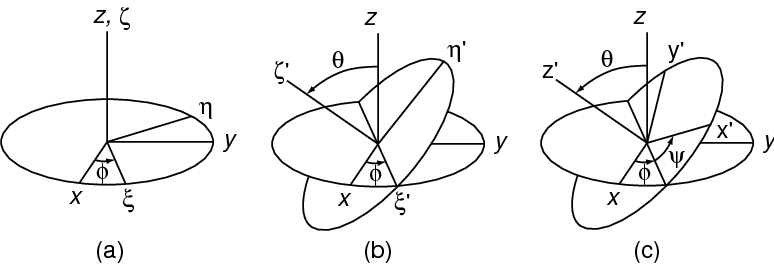
\includegraphics[width=0.75\textwidth]{images/euler-angles}
\end{figure}

The Lagrangian for a rigid bod spinning about a fixed pivot is 
\begin{equation*}
\lag = \f{1}{2}\lambda_1(\dot{\phi}^2\sin^2\theta + \dot{\theta}^2) + \f{1}{2}\lambda_3(\dot{\psi} + \dot{\phi}\cos\theta)^2 - MgR\cos\theta
\end{equation*}








\section{Coupled Oscillators and Normal Modes}


The configuration of a system with $n$ degrees of freedom can be specified by an $n\times 1$ column matrix $\mathbf{q}$ of generalized coordinates $q_i$. For small oscillations near a stable equilibrium (with coordinates chosen so that $\mathbf{q} = 0$ at equilibrium), the equation of motion has the form 
\begin{equation}
\mathbf{M} \ddot{\mathbf{q}} = -\mathbf{K} \mathbf{q}. 
\end{equation}
Here $\mathbf{M}$ and $\mathbf{K}$ are the \textbf{mass} and \textbf{spring-constant matrices}, respectively. Their matrix elements can be obtained by writing out the kinetic and potential energies into the forms:
\begin{equation*}
T = \f{1}{2}\sum_{j,k} M_{jk} \dot{q}_j \dot{q}_k \quad \text{and} \quad U = \f{1}{2}\sum_{j,k} K_{jk}q_jq_k.
\end{equation*} 
Sometimes one may forget these forms. To recover them, either write out the equations of motion explicitly, or use dimensional analysis. A possible problem with trying to remember these things is the factor of $1/2$. My recommendation when you have a lot of time left on the exam is to work out the equations of motion explicitly, be it from Newtonian or Lagrangian mechanics, and then rearrange and get the matrix equation above. \\


A \textbf{normal mode} is any motion in which all $n$ coordinates oscillation sinusoidally with the same frequency $\omega$ (a \textbf{normal/eigen-frequency}) and can be written as 
\begin{equation*}
\mathbf{q}(t) = \Re\{ \mathbf{a} e^{i\omega t} \} \implies \ddot{\mathbf{q}} = -\omega^2 \mathbf{q},
\end{equation*}
where 
\begin{equation*}
\lp \mathbf{K} - \omega^2 \mathbf{M} \rp \mathbf{a} = \mathbf{0}
\end{equation*}


For any system with $n$ degrees of freedom and a stable equilibrium at $\mathbf{q} = 0$, there are $n$ normal frequencies $\omega_1,\dots, \omega_n$ (not necessarily distinct) and $n$ linearly independent eigenvectors $\mathbf{a}_1,\dots, \mathbf{a}_n$ spanning the configuration space of the system. \\


When any solution is expanded in terms of the normal modes, the expansion coefficients $\xi_i(t)$ are called \textbf{normal coordinates}, and each oscillates at the corresponding eigenfrequency $\omega_i$.






\section{Collision Theory}

The \textbf{scattering angle} is the angle $\theta$ by which the projectile is deflected in its counter with a target. The \textbf{impact parameter} $b$ is the distance by which the projectile would have missed the center of the target if it had been undeflected. \\


The \textbf{cross section} $\sigma_\text{oc}$ for a particular outcome (oc) (elastic scattering, absorption, reaction, fission) is defined by 
\begin{equation*}
N_\text{oc} = N_\text{inc} n_\text{tar} \sigma_\text{oc}.
\end{equation*}
$N_\text{oc}$ is the number of outcomes of the type considered, $N_\text{inc}$ is the number of incident projectiles, and $n_\text{tar}$ is the density (number/area) of targets. \\


The \textbf{differential cross section} $d\sigma/d\Omega (\theta,\phi)$ for scattering in a direction $(\theta,\phi)$ is defined by 
\begin{equation*}
N_\text{sc, into $d\Omega$} = N_\text{inc} n_\text{tar} \f{d\sigma}{d\Omega}(\theta,\phi) \,d\Omega.
\end{equation*}



If you can find the scattering angle as a function of the impact parameter $b$ or vice versa then 
\begin{equation*}
\f{d\sigma}{d\Omega} = \f{b}{\sin\theta} \abs{\f{db}{d\theta}}.
\end{equation*}



\section{Special Relativity}


\noindent \textbf{Time dilation:}
\begin{equation*}
\Delta t' = \gamma \Delta t
\end{equation*}
where $\gamma = 1/\sqrt{1-\beta^2}$, $\be = v/c$. $v$ is the speed of $\mathcal{S}'$ relative to $\mathcal{S}$.

\noindent \textbf{Length contraction:}
\begin{equation*}
l = l_0/\gamma.
\end{equation*}


\noindent \textbf{The Lorentz transformation:}
\begin{equation*}
\begin{pmatrix}
ct' \\ x' \\ y' \\ z'
\end{pmatrix}
= 
\begin{pmatrix}
\gamma & -\be\gamma &&\\
-\be \gamma & \gamma &&\\
&&1&\\
&&&1
\end{pmatrix}
\begin{pmatrix}
ct\\x\\y\\z
\end{pmatrix}
\end{equation*}



\noindent \textbf{Addition of velocities}
\begin{equation*}
v_x' = \f{v_x - v}{1 - v_x v/c^2},\quad v_y' = \f{v_y}{\gamma(1 - v_xv/c^2)}, \quad v_z' = \f{v_z}{\gamma(1 - v_x v/c^2)}
\end{equation*}


\noindent \textbf{The Relativistic Doppler Effect:}
Light from a source traveling with velocity $\textbf{v}$ relative to frame $\mathcal{S}$ is observed at an angle $\theta$. If the frequency of the light as measured in the source's rest frame is $\omega_0$ then the frequency observed in $\mathcal{S}$ is 
\begin{equation*}
\omega = \f{\omega_0}{\gamma(1- \beta\cos\theta)}.
\end{equation*}




\noindent \textbf{Mass, Four-velocity, Momentum, and Energy:}
The \textbf{invariant mass} is the rest mass. The \textbf{four-velocity} is 
\begin{equation*}
u = \f{dx}{dt_0} = \gamma(c,\textbf{v}).
\end{equation*}


\noindent \textbf{Useful Relations:}

\begin{equation*}
p\cdot p = m^2c^2
\end{equation*}

\begin{equation*}
E^2 = m^2 c^4 + p^2 c^2
\end{equation*}



\noindent \textbf{Three-force:}

\begin{equation*}
\textbf{F} = \f{d \textbf{p}}{dt}
\end{equation*}


\noindent \textbf{Four-force:}

\begin{equation*}
\textbf{K} = \f{dp}{dt_0}
\end{equation*}



\noindent \textbf{Massless Particles:}
\begin{equation*}
E = pc,\quad v = c, \quad p^2 = 0.
\end{equation*}




\noindent \textbf{Transformation of the EM fields:} Assume motion along the $x$-axis.


\begin{align*}
&E_x' = E_x, \quad E_y' = \gamma(E_y - v B_z), \quad E_z' = \gamma(E_z + vB_y)\\
&B_x' = B_x, \quad B_y' = \gamma\lp B_y + \f{v}{c^2} E_z\rp, \quad B_z' = \gamma(B_z - \f{v}{c^2} E_y).
\end{align*}




\section{Miscellaneous Factoids}

\subsection{}

The Lagrangian for a charge in an electromagnetic field is 
\begin{equation*}
\lag(\mathbf{r}, \dot{\mathbf{r}},t) = \f{1}{2}m \dot{\mathbf{r}}^2 - q(V - \dot{\mathbf{r}}\cdot \mathbf{A}).
\end{equation*}




\chapter{Problems}




\bibliography{Bui_AMO} 
\bibliographystyle{ieeetr}


\end{document}